%==============================================================================
%  CHAPITRE 3 — Modélisation et Conception du framework EmoLearn
%  Contenu SEUL (à inclure via \input / \include dans le document principal).
%  Aucun préambule ici : voir la note en tête de fichier pour les paquets requis.
%------------------------------------------------------------------------------
%  Paquets à avoir dans le préambule du document principal :
%    \usepackage{tikz}
%    \usetikzlibrary{arrows.meta,positioning,shapes.geometric,calc,fit,backgrounds}
%    \usepackage{float}
%    \usepackage{booktabs}
%    \usepackage{longtable}   % ou ltablex (déjà présent dans votre template)
%    \usepackage{enumitem}
%    \usepackage[backend=biber,style=numeric-comp,sorting=nyt,maxbibnames=99]{biblatex}
%  Références à ajouter dans references.bib : gupta2016daisee, busso2008iemocap,
%    hevner2004design, lewis2020retrieval, touvron2023llama, brown2020language,
%    kasneci2023chatgpt, dmello2012dynamics, pekrun2006control.
%  (Définir aussi \newcommand{\emolearn}{\textsc{EmoLearn}} dans le préambule.)
%==============================================================================

\chapter{Modélisation et Conception du framework EmoLearn}
\label{chap:conception}
\minitoc

\par L'état de l'art a mis en évidence un espace de conception encore peu exploré :
celui d'un dispositif reliant, au sein d'une même chaîne, la \emph{perception}
multimodale de l'engagement, une \emph{décision} pédagogique explicite et la
\emph{génération} automatique de contenu adaptatif. Ce chapitre présente la
modélisation et la conception du framework \emolearn{} qui matérialise cette
articulation. Nous exposons d'abord le cadre conceptuel et l'architecture
globale (section~\ref{sec:framework}), puis l'analyse du corpus \textsc{DAiSEE}
qui constitue le socle du système (section~\ref{sec:daisee}) et le positionnement
du corpus \textsc{IEMOCAP} en modalité vocale complémentaire
(section~\ref{sec:iemocap}). Nous détaillons ensuite le c\oe ur scientifique du travail — le modèle
engagement\,$\rightarrow$\,adaptation (section~\ref{sec:modele}) — avant de
décrire le système de génération fondé sur des patrons de prompts
(section~\ref{sec:generation}) et, enfin, la conception du prototype de
simulation (section~\ref{sec:prototype}).

%==============================================================================
\section{Framework conceptuel proposé}
\label{sec:framework}

\subsection{Architecture globale du système}

\emolearn{} est conçu comme une chaîne de traitement organisée en trois couches
fonctionnelles successives, conformément à la démarche de recherche orientée
conception adoptée dans ce mémoire \cite{hevner2004design}. Chaque couche répond
à une question distincte :

\begin{description}
  \item[Couche de perception — \og Que ressent l'apprenant ? \fg] Elle estime
  l'état d'engagement à partir de deux modalités : le \textbf{visage}, via un
  module de reconnaissance des expressions faciales (FER) appliqué au corpus
  \textsc{DAiSEE} \cite{gupta2016daisee}, et la \textbf{voix}, via un module de
  reconnaissance des émotions vocales (SER) appliqué au corpus \textsc{IEMOCAP}
  \cite{busso2008iemocap}. Un \textbf{module de fusion} combine ensuite les deux
  estimations et gère les situations de conflit.

  \item[Couche de décision — \og Faut-il intervenir, et comment ? \fg] Elle
  applique, sur l'état fusionné et son historique temporel, un ensemble de règles
  qui déterminent (i)~s'il convient de déclencher une adaptation, (ii)~le type de
  contenu pédagogique approprié et (iii)~le patron de génération précis à
  mobiliser.

  \item[Couche de génération — \og Quel contenu produire ? \fg] Elle construit un
  prompt contextuel structuré à partir du patron retenu, éventuellement enrichi
  par un mécanisme de récupération documentaire (RAG), puis sollicite un grand
  modèle de langue pour produire le contenu adaptatif final.
\end{description}

La figure~\ref{fig:architecture} présente cette architecture en couches et les
modules qui la composent. Un principe de conception structurant mérite d'être
souligné : le \textbf{moteur de fusion} et le \textbf{moteur de décision} sont
\emph{uniques} et partagés entre le pipeline de production (génération de contenu)
et le banc d'essai de validation. Ce choix garantit que ce qui est évalué
expérimentalement correspond exactement à ce qui est utilisé en fonctionnement.

\begin{figure}[H]
\centering
\begin{tikzpicture}[
  font=\footnotesize,
  mod/.style={rectangle, rounded corners, draw=black, thick, align=center,
              text width=2.7cm, minimum height=1.0cm, fill=white},
  layer/.style={rectangle, rounded corners, draw=black!35, thick, inner sep=10pt},
  io/.style={rectangle, draw=black!55, dashed, align=center, text width=3.2cm,
             minimum height=0.9cm},
  arr/.style={-{Stealth[length=2.6mm]}, thick}
]
% Entrée
\node[io] (in) {Clip vidéo DAiSEE + segment audio + contexte pédagogique};

% Couche perception
\node[mod, below left=1.0cm and 0.2cm of in] (fer) {Module FER — visage\\vote multi-frames\\+ mapping appris};
\node[mod, below right=1.0cm and 0.2cm of in] (ser) {Module SER — voix\\heuristique\\ou tête apprise};
\node[mod, below=3.0cm of in] (fus) {Fusion multimodale\\pedagogical priority\\or weighted vote};

% Couche décision
\node[mod, below=1.0cm of fus] (temp) {Règles temporelles\\(déclenchement)};
\node[mod, right=0.6cm of temp] (dec) {Moteur de décision\\(type + template)};

% Couche génération
\node[mod, below=1.0cm of temp] (rag) {RAG (optionnel)\\récupération};
\node[mod, right=0.6cm of rag] (llm) {LLM Groq\\(Llama 3.1)};

% Sortie
\node[io, below=1.0cm of rag, xshift=1.6cm] (out) {Contenu adaptatif + journal de décision};

\draw[arr] (in) -- (fer);
\draw[arr] (in) -- (ser);
\draw[arr] (fer) -- (fus);
\draw[arr] (ser) -- (fus);
\draw[arr] (fus) -- (temp);
\draw[arr] (fus) -- (dec);
\draw[arr] (temp) -- (dec);
\draw[arr] (dec) -- (llm);
\draw[arr] (rag) -- (llm);
\draw[arr] (llm) -- (out);

\begin{scope}[on background layer]
\node[layer, fit=(fer)(ser)(fus), label={[align=left]left:\rotatebox{90}{\textbf{Perception}}}] {};
\node[layer, fit=(temp)(dec), label={[align=left]left:\rotatebox{90}{\textbf{Décision}}}] {};
\node[layer, fit=(rag)(llm), label={[align=left]left:\rotatebox{90}{\textbf{Génération}}}] {};
\end{scope}
\end{tikzpicture}
\caption{Architecture en couches d'\emolearn{} : perception multimodale,
décision pédagogique et génération de contenu.}
\label{fig:architecture}
\end{figure}

\subsection{Workflow de génération adaptative}
\label{subsec:workflow}

Le traitement d'un clip suit un enchaînement déterministe de sept étapes, résumé
ci-dessous et implémenté dans le module \texttt{pipeline} du prototype :

\begin{enumerate}[label=\textbf{\arabic*.}]
  \item \textbf{Acquisition.} Le \textbf{fichier vidéo} du clip \textsc{DAiSEE} est
  résolu sur disque à partir de son identifiant, puis associé au segment audio
  apparié et à un contexte pédagogique (concept, module, niveau de l'apprenant,
  moment du cours).
  \item \textbf{Perception unimodale.} Le module FER décode la vidéo, y détecte le
  visage sur plusieurs images réparties sur la durée du clip, agrège leurs
  distributions d'émotions par \emph{vote multi-frames}, puis estime l'état facial
  et son niveau ; le module SER estime en parallèle l'état vocal à partir de la
  forme d'onde du signal audio.
  \item \textbf{Fusion.} Les deux estimations sont combinées (pondération
  60\,\%~/~40\,\%) et les conflits éventuels sont résolus (section~\ref{sec:modele}).
  \item \textbf{Analyse temporelle.} L'historique récent des clips est examiné
  pour décider de l'urgence et du \emph{déclenchement} d'une adaptation.
  \item \textbf{Décision.} Si une intervention est requise, le moteur détermine
  la stratégie, le type de contenu (A/B/C/D) et le patron précis (A1--D5).
  \item \textbf{Génération.} Un prompt contextuel structuré est construit à partir
  du patron, éventuellement enrichi par le RAG, puis soumis au LLM.
  \item \textbf{Restitution et traçabilité.} Le contenu produit est renvoyé à
  l'interface et chaque décision est journalisée (état, stratégie, patron,
  paramètres de fusion) pour analyse ultérieure.
\end{enumerate}

Lorsque l'analyse temporelle conclut à un engagement stable, aucune génération
n'est déclenchée : le système signale explicitement une \emph{non-intervention},
ce qui évite de sur-solliciter l'apprenant et documente le choix de ne rien faire.

\paragraph{Perception sur le signal, annotations réservées à la vérité terrain.}
Un choix de conception mérite d'être explicité ici, car il conditionne la validité
de tout ce qui suit : la couche de perception opère sur le \textbf{signal brut} et
non sur les annotations du corpus. Le module FER ouvre le fichier vidéo du clip,
y détecte le visage image par image et produit ses propres distributions
d'émotions ; le module SER analyse de la même manière la forme d'onde du segment
audio. Les niveaux d'engagement annotés dans \textsc{DAiSEE} ne sont à aucun
moment fournis en entrée de la perception : ils tiennent exclusivement le rôle
d'\textbf{étiquettes de référence}, d'une part pour entraîner les mises en
correspondance apprises (sections~\ref{subsec:fer-appris}
et~\ref{subsec:ser-appris}), d'autre part pour mesurer les performances lors de la
validation. Un système qui lirait les annotations pour \emph{estimer} l'état
n'évaluerait que lui-même ; le prototype ne comporte donc aucune voie d'entrée
alternative — ni téléversement d'image, ni saisie manuelle d'un état — et l'unique
entrée de la chaîne reste le couple \emph{(clip vidéo, segment audio)}.

%==============================================================================
\section{Analyse du dataset DAiSEE}
\label{sec:daisee}

\subsection{Description et caractéristiques}

Le corpus \textsc{DAiSEE} (\emph{Dataset for Affective States in E-Environments})
\cite{gupta2016daisee} est un jeu de données vidéo de référence pour la
reconnaissance de l'engagement \og dans la nature \fg{} (\emph{in the wild}). Il
rassemble environ 9\,000 clips vidéo d'une dizaine de secondes chacun, capturés
auprès d'étudiants en situation réelle d'apprentissage en ligne, dans des
conditions variées d'éclairage et d'arrière-plan. Chaque clip est annoté selon
\textbf{quatre états affectifs} — l'ennui (\emph{boredom}), la confusion
(\emph{confusion}), l'engagement (\emph{engagement}) et la frustration
(\emph{frustration}) — chacun exprimé sur une échelle ordinale à
\textbf{quatre niveaux d'intensité} (0~: très faible, 1~: faible, 2~: élevé,
3~: très élevé). Le tableau~\ref{tab:daisee-etats} synthétise cette taxonomie,
qui constitue le référentiel de tout le projet.

\begin{table}[H]
\centering
\renewcommand{\arraystretch}{1.2}
\begin{tabular}{>{\bfseries}l p{9.5cm}}
\toprule
État & Signification dans le contexte d'apprentissage \\
\midrule
Engagement  & Attention active et implication dans la tâche d'apprentissage. \\
Boredom     & Ennui, désengagement passif, baisse de la stimulation. \\
Confusion   & Incompréhension d'un concept, difficulté de traitement. \\
Frustration & Blocage émotionnel, tension liée à une difficulté persistante. \\
\bottomrule
\end{tabular}
\caption{Les quatre états affectifs annotés dans \textsc{DAiSEE}
(niveaux d'intensité 0 à 3).}
\label{tab:daisee-etats}
\end{table}

Concrètement, chaque enregistrement du corpus est identifié par un
\texttt{ClipID} et associé à un quadruplet de scores
$(\text{Boredom}, \text{Confusion}, \text{Engagement}, \text{Frustration})$.
Ce format tabulaire est directement exploité par le prototype pour la simulation
des parcours d'apprentissage.

\subsection{Distribution des états d'engagement}

L'analyse de la distribution des annotations révèle un \textbf{déséquilibre de
classes marqué}, caractéristique bien documentée de \textsc{DAiSEE}. L'engagement
est l'état largement dominant : la majorité des clips présentent un niveau
d'engagement élevé (2 ou 3), tandis que les états négatifs — confusion et surtout
frustration — sont concentrés sur les niveaux faibles (0 ou 1), les niveaux
intenses étant rares. Ce déséquilibre a deux conséquences directes pour la
conception :

\begin{itemize}[leftmargin=1.4em]
  \item les états \emph{critiques} (confusion et frustration élevées), pourtant
  les plus importants sur le plan pédagogique, sont \textbf{sous-représentés} ;
  \item une simple maximisation de l'exactitude globale tendrait à privilégier la
  classe majoritaire (engagement) au détriment de la détection des états à risque.
\end{itemize}

Ce constat justifie un choix de conception assumé dans tout le système : accorder
une \textbf{priorité pédagogique} aux états négatifs, afin de ne jamais masquer un
apprenant en difficulté derrière un score d'engagement équivalent
(section~\ref{sec:modele}). La distribution détaillée (histogrammes par état et
par niveau) est produite par l'analyse exploratoire (livrable OS1) ; la
figure~\ref{fig:distribution} en accueillera la restitution graphique.

\begin{figure}[H]
\centering
% Remplacez par la figure produite par votre notebook OS1 (dossier figures/)
% 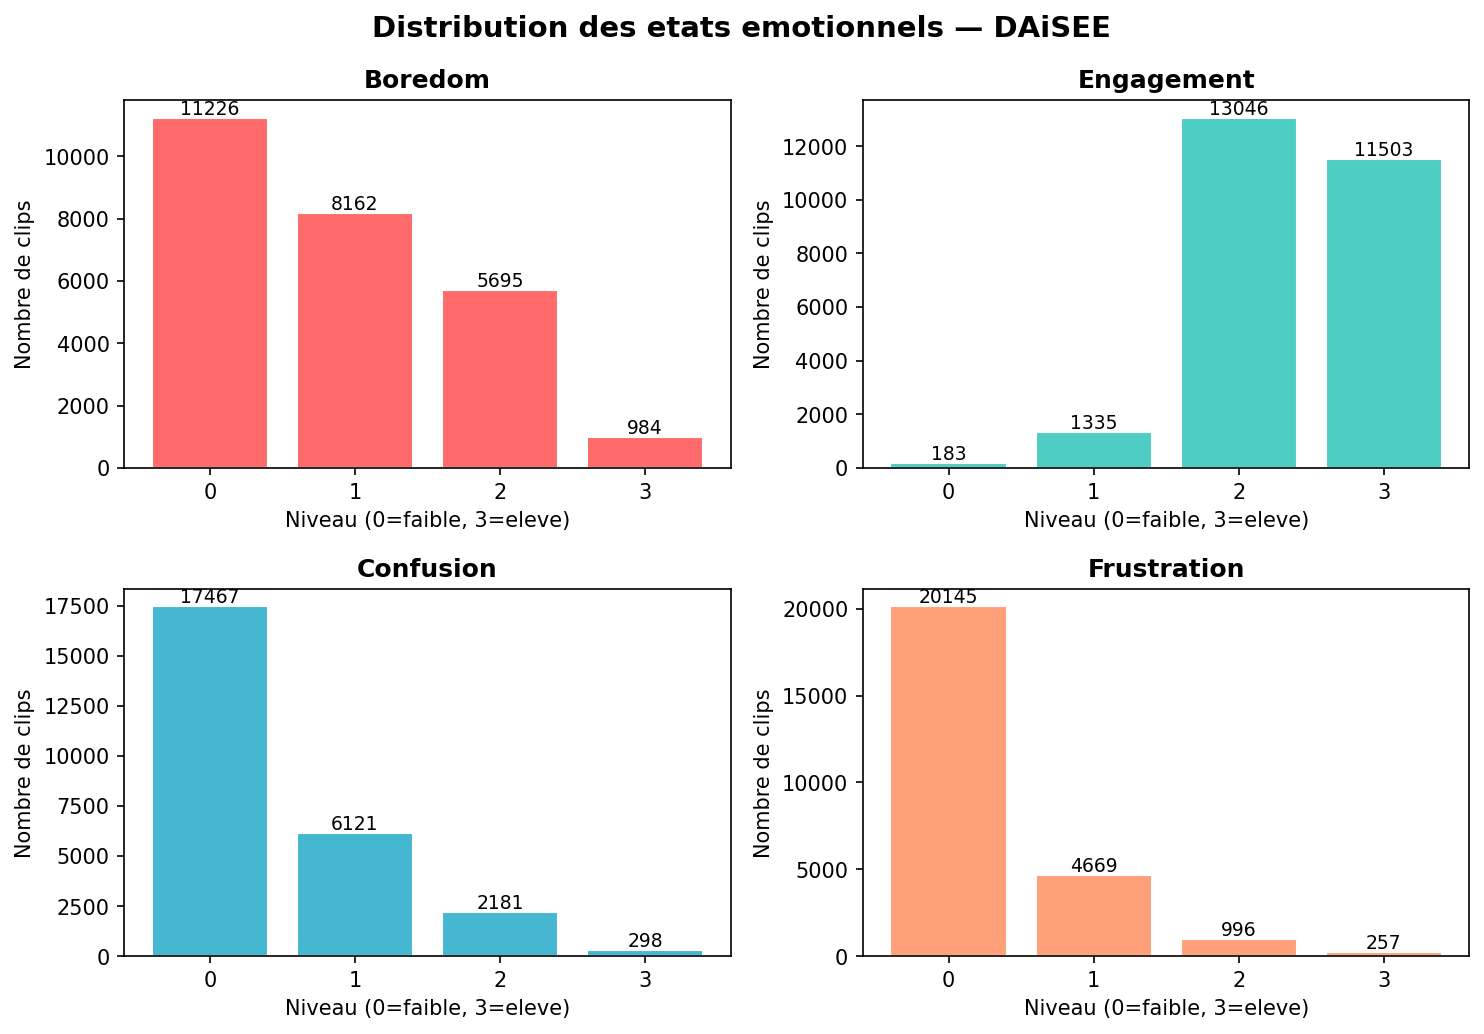
\includegraphics[width=0.9\textwidth]{figures/daisee_distribution.png}
\fbox{\parbox[c][3.2cm][c]{0.9\textwidth}{\centering\itshape
Emplacement réservé à l'histogramme de distribution des quatre états
DAiSEE par niveau d'intensité (issu de l'analyse exploratoire OS1).}}
\caption{Distribution des états d'engagement dans \textsc{DAiSEE}
(à insérer depuis le notebook d'analyse exploratoire).}
\label{fig:distribution}
\end{figure}

\subsection{Analyse exploratoire des données}

L'analyse exploratoire poursuit trois objectifs. Premièrement, \textbf{caractériser
les co-occurrences} entre états : les données montrent que l'engagement varie en
sens inverse de l'ennui, tandis que la confusion et la frustration tendent à
coexister — motif cohérent avec la dynamique affective décrite dans la littérature
sur l'apprentissage \cite{dmello2012dynamics,pekrun2006control}. Deuxièmement,
\textbf{déterminer l'état dominant} de chaque clip : le prototype retient l'état
de score maximal, avec une règle de départage explicite en cas d'égalité
(priorité~: Frustration~$>$~Confusion~$>$~Boredom~$>$~Engagement), afin de rester
cohérent avec la priorité pédagogique. Troisièmement, \textbf{constituer un
sous-ensemble représentatif} : une sélection de scénarios (clips isolés) et de
parcours (séquences de plusieurs clips) est extraite pour alimenter la simulation.

\subsection{Identification de patterns critiques}

Au-delà de l'état instantané, la conception introduit la notion de \textbf{pattern
pédagogique}, qui qualifie la situation globale d'un clip ou d'une séquence et
oriente ensuite le choix du patron de génération. Le tableau~\ref{tab:patterns}
récapitule les patterns retenus et leurs conditions de déclenchement.

\begin{table}[H]
\centering
\renewcommand{\arraystretch}{1.2}
\begin{tabular}{>{\bfseries}l p{9.2cm}}
\toprule
Pattern & Condition (scores DAiSEE) \\
\midrule
critique          & Au moins trois états simultanément $\geq 2$ (situation cumulée). \\
engagement\_faible & Engagement $\leq 1$, sans confusion ni frustration marquées. \\
confusion         & État dominant = Confusion. \\
ennui\_eleve       & État dominant = Boredom. \\
frustration       & État dominant = Frustration. \\
stable            & Engagement dominant, situation acceptable. \\
\bottomrule
\end{tabular}
\caption{Patterns pédagogiques dérivés des scores DAiSEE.}
\label{tab:patterns}
\end{table}

%==============================================================================
\section{Positionnement et usage du corpus IEMOCAP}
\label{sec:iemocap}

\textsc{IEMOCAP} (\emph{Interactive Emotional Dyadic Motion Capture})
\cite{busso2008iemocap} constitue le \textbf{second jeu de données} mobilisé par
\emolearn{}. Contrairement à \textsc{DAiSEE}, il ne fonde pas la taxonomie
pédagogique : il apporte la \textbf{modalité vocale} et, dans un cadre distinct,
un \textbf{sous-corpus audiovisuel aligné} pour la validation de la fusion. Cette
section précise ce rôle complémentaire, la projection des émotions conversationnelles
vers l'espace \textsc{DAiSEE}, l'appariement opéré dans le pipeline produit et le
banc d'essai Option~A.

\subsection{Complémentarité avec \textsc{DAiSEE}}

Les deux corpus couvrent des contextes et des modalités distincts, mais convergent
vers la même taxonomie d'engagement à quatre états (tableau~\ref{tab:daisee-etats}).
Le tableau~\ref{tab:complementarite-corpus} résume cette complémentarité.

\begin{table}[H]
\centering
\renewcommand{\arraystretch}{1.2}
\begin{tabular}{>{\bfseries}l p{5.2cm} p{5.2cm}}
\toprule
Aspect & \textsc{DAiSEE} & \textsc{IEMOCAP} \\
\midrule
Contexte & Apprenants en e-learning (\emph{in the wild}) &
Dialogues actés, dyades (sessions 1--5) \\
Modalité principale & Visage / engagement annoté &
Voix (+ vidéo pour le banc d'essai) \\
Étiquettes natives & 4 états $\times$ niveaux 0--3 &
Émotions discrètes + dimensions VAD \\
Rôle dans \emolearn{} &
Socle : scénarios, patterns, décision &
Voix en production ; validation AV alignée \\
\bottomrule
\end{tabular}
\caption{Complémentarité des corpus \textsc{DAiSEE} et \textsc{IEMOCAP} dans
\emolearn{}.}
\label{tab:complementarite-corpus}
\end{table}

\subsection{Description et caractéristiques}

\textsc{IEMOCAP} rassemble des enregistrements audiovisuels de dialogues entre
deux acteurs, annotés au niveau de l'\emph{utterance} (segment de parole) par des
émotions discrètes (codes sur deux à quatre lettres) et par des scores
valence--activation--dominance (VAD). Le corpus parsé du projet compte 10\,039 utterances, chacune associée à un fichier audio réel
(couverture \emph{wav} intégrale dans ce dépôt). Les annotations sont exploitées
via un fichier tabulaire intermédiaire (\texttt{iemocap\_parsed.csv}) produit par
un parseur dédié, puis consommées par le module SER (section~\ref{subsec:ser-appris}).

\subsection{Projection des émotions vers la taxonomie \textsc{DAiSEE}}
\label{subsec:mapping-iemocap}

Les émotions conversationnelles d'\textsc{IEMOCAP} ne coïncident pas
naturellement avec les états d'engagement en apprentissage mesurés par
\textsc{DAiSEE}. La conception retient donc une \textbf{table de projection}
(documentée dans \texttt{mapping\_iemocap\_daisee.csv}), qui traduit chaque code
émotionnel en état \textsc{DAiSEE} et en niveau d'intensité typique
(tableau~\ref{tab:mapping-iemocap}). Cette correspondance est une
\textbf{hypothèse de construit}, et non une équivalence psychologique démontrée :
elle rend le pipeline cohérent en ramenant visage et voix dans un espace commun,
mais elle doit être discutée et, si possible, \emph{mesurée} (voir
section~\ref{subsec:sensibilite-mapping}).

\begin{table}[H]
\centering
\renewcommand{\arraystretch}{1.15}
\begin{tabular}{>{\bfseries}l l c p{4.8cm}}
\toprule
Code IEMOCAP & État DAiSEE & Niv. & Justification pédagogique \\
\midrule
hap, exc & Engagement  & 3 & Valence positive, activation forte \\
neu      & Boredom     & 1 & Neutre prolongé $\approx$ faible stimulation \\
sad      & Boredom     & 2 & Faible engagement \\
ang, fru & Frustration & 3 & Blocage, tension \\
dis      & Frustration & 2 & Rejet, gêne modérée \\
sur, fea & Confusion   & 2--3 & Incertitude, surprise cognitive \\
xxx      & Boredom     & 1 & Non classifié $\rightarrow$ défaut prudent \\
\bottomrule
\end{tabular}
\caption{Projection de référence des émotions \textsc{IEMOCAP} vers la taxonomie
\textsc{DAiSEE} (hypothèse de travail).}
\label{tab:mapping-iemocap}
\end{table}

\subsection{Appariement voix--scénarios dans le pipeline produit}
\label{subsec:appariement}

Dans la chaîne de \textbf{production} (simulation sur clips \textsc{DAiSEE}), le
visage et la voix ne proviennent pas du même individu : le module FER analyse un
clip \textsc{DAiSEE}, tandis que le module SER sélectionne une utterance
\textsc{IEMOCAP} \emph{émotionnellement cohérente} avec l'état dominant du
scénario. La règle retenue est la suivante :
\begin{enumerate}[label=\textbf{\arabic*.}, leftmargin=1.6em]
  \item calcul de l'état dominant du scénario \textsc{DAiSEE} ;
  \item filtrage des utterances \textsc{IEMOCAP} projetées sur le \emph{même} état ;
  \item sélection reproductible via l'identifiant du scénario
        (\texttt{scenario\_id \% pool\_size}), garantissant qu'un même scénario
        produit toujours la même voix ;
  \item analyse du segment audio réel \texttt{[start\_time, end\_time]} extrait
        du fichier dialogue \texttt{.wav}.
\end{enumerate}

Cet appariement améliore la \emph{cohérence émotionnelle} visage/voix par rapport
à un tirage aléatoire, mais conserve une limite assumée : \textbf{absence de
synchronisation temporelle} entre l'apprenant filmé (\textsc{DAiSEE}) et le locuteur
enregistré (\textsc{IEMOCAP}). Cette tension est levée uniquement dans le banc
d'essai décrit ci-dessous.

\subsection{Sous-corpus audiovisuel aligné (Option~A)}
\label{subsec:option-a}

Pour \textbf{valider la fusion multimodale} sans l'appariement hétérogène du
pipeline produit, un sous-corpus \textsc{IEMOCAP} \textbf{audiovisuel aligné} est
construit hors ligne : pour chaque utterance retenue, le \textbf{visage} et la
\textbf{voix proviennent du même locuteur}, synchronisés sur le segment annoté
(module \texttt{iemocap\_video}, extraction multi-frames + SER sur le même intervalle).
Les vidéos dyadiques (720$\times$480) imposent une règle de crop : le visage du
locuteur est extrait de la moitié gauche ou droite de l'image selon qu'il porte
ou non les marqueurs mocap. Ce banc d'essai partage le \textbf{même moteur de fusion}
que la production ; seules les entrées changent. Les métriques comparatives (modalités
unimodales vs fusion, \emph{pedagogical priority} vs \emph{weighted vote}) sont
présentées au chapitre~5.

\subsection{Analyse de sensibilité du mapping}
\label{subsec:sensibilite-mapping}

La robustesse de la projection émotion $\rightarrow$ engagement est évaluée par une
\textbf{analyse de sensibilité} sur l'ensemble des 10\,039 utterances : on mesure
l'impact de ré-interprétations plausibles du mapping (tableau~\ref{tab:sensibilite-mapping}).
Les variantes affectant \texttt{neu} (neutre $\rightarrow$ Engagement au lieu de
Boredom) ou \texttt{sad} (tristesse $\rightarrow$ Frustration) modifient jusqu'à
17\,\% et 10,8\,\% des étiquettes projetées, confirmant que cette hypothèse n'est
pas anodine. Le protocole complet et la discussion sont détaillés au chapitre~5.

\begin{table}[H]
\centering
\renewcommand{\arraystretch}{1.2}
\begin{tabular}{>{\bfseries}l p{7.2cm} r}
\toprule
Variante testée & Modification du mapping & Utterances changées \\
\midrule
neu\_engagement &
\texttt{neu} $\rightarrow$ Engagement (au lieu de Boredom) & 17,0\,\% \\
sad\_frustration &
\texttt{sad} $\rightarrow$ Frustration (au lieu de Boredom) & 10,8\,\% \\
surprise\_engagement &
\texttt{sur} $\rightarrow$ Engagement (au lieu de Confusion) & 1,1\,\% \\
disgust\_boredom &
\texttt{dis} $\rightarrow$ Boredom (au lieu de Frustration) & 0,0\,\% \\
\bottomrule
\end{tabular}
\caption{Sensibilité du mapping \textsc{IEMOCAP} $\rightarrow$ \textsc{DAiSEE}
(sur 10\,039 utterances).}
\label{tab:sensibilite-mapping}
\end{table}

%==============================================================================
\section{Modèle engagement-adaptation}
\label{sec:modele}

Le modèle engagement\,$\rightarrow$\,adaptation constitue le c\oe ur scientifique
du framework. Il transforme un état perçu en une décision pédagogique traçable, à
travers quatre composants : une taxonomie des états, un mapping vers des besoins
pédagogiques, des règles de déclenchement temporel et des stratégies par état.

\subsection{Taxonomie des états et mise en correspondance du signal facial}

La perception s'appuie sur la taxonomie \textsc{DAiSEE} à quatre états
(tableau~\ref{tab:daisee-etats}). Les émotions produites par les modules FER
(sept classes) et SER sont d'abord ramenées dans cet espace commun. Cette mise en
correspondance est conçue à \textbf{deux niveaux} : une table fixe, lisible et
justifiable \emph{a priori}, qui sert de référence ; et un modèle \emph{appris}
sur les données, qui la remplace lorsqu'il apporte un gain mesuré. Le
tableau~\ref{tab:fer-mapping} présente le premier niveau pour le visage.

\begin{table}[H]
\centering
\renewcommand{\arraystretch}{1.15}
\begin{tabular}{>{\bfseries}l l c}
\toprule
Émotion faciale & État DAiSEE & Niveau associé \\
\midrule
happy    & Engagement  & 3 \\
neutral  & Boredom     & 1 \\
sad      & Boredom     & 2 \\
angry    & Frustration & 3 \\
fear     & Confusion   & 3 \\
surprise & Confusion   & 2 \\
disgust  & Frustration & 2 \\
\bottomrule
\end{tabular}
\caption{Mapping heuristique de référence des émotions faciales (FER) vers les
états DAiSEE.}
\label{tab:fer-mapping}
\end{table}

\subsection{Apprentissage du mapping visage $\rightarrow$ engagement}
\label{subsec:fer-appris}

La table~\ref{tab:fer-mapping} traduit un raisonnement pédagogique — un visage en
colère signale une frustration, un visage neutre l'amorce d'un désengagement —
mais elle n'est calibrée sur aucune donnée. La conception prévoit donc un second
mode, retenu par défaut à l'exécution, dans lequel cette correspondance est
\textbf{apprise} sur \textsc{DAiSEE}.

Le principe est celui d'un apprentissage volontairement \emph{léger} : le réseau
de reconnaissance faciale pré-entraîné n'est pas ré-entraîné, seul le lien entre
ses sorties et la taxonomie d'engagement l'est. Le vecteur des sept scores
d'émotion produit par le modèle pré-entraîné constitue le vecteur de
caractéristiques, et l'état \textsc{DAiSEE} annoté du clip constitue l'étiquette
cible. Un \textbf{Random Forest} (scikit-learn) est entraîné sur ce couple,
ses hyperparamètres — \texttt{n\_estimators}, \texttt{max\_depth} — étant sélectionnés
par \textbf{GridSearchCV} avec \emph{stratified cross-validation}. Ce choix
d'algorithme se justifie par la faible dimension du problème (sept variables
explicatives), par la nature non linéaire de la relation recherchée et par un coût
de calcul compatible avec les moyens d'un travail de master.

Un \textbf{garde-fou} est intégré à la sélection du mode : le modèle appris n'est
préféré à l'heuristique que s'il améliore \emph{à la fois} l'exactitude globale et
le F-score macro. Cette double condition n'est pas cosmétique. Comme le montre la
section~\ref{sec:daisee}, \textsc{DAiSEE} est fortement déséquilibré en faveur de
l'engagement ; un modèle qui prédirait systématiquement la classe majoritaire
afficherait une exactitude flatteuse tout en étant pédagogiquement inutile,
puisqu'il ne détecterait jamais un apprenant en difficulté. Exiger un gain
simultané sur une métrique sensible aux classes rares rend ce phénomène visible
plutôt que de le laisser passer pour une performance. Le chapitre~5 quantifie
précisément ce risque sur le modèle effectivement entraîné.

Les deux modes demeurent interchangeables par configuration — heuristique
(référence), appris (défaut), ou sélection automatique conditionnée au gain
mesuré. La table~\ref{tab:fer-mapping} conserve ainsi le statut explicite de
\textbf{baseline}, et non celui d'une vérité posée.

\subsection{Perception vocale : heuristique acoustique et tête apprise}
\label{subsec:ser-appris}

Le module vocal suit la même logique à deux niveaux. La \textbf{méthode
heuristique} sert de référence : elle extrait du signal un jeu de descripteurs
acoustiques classiques — énergie moyenne, taux de passage par zéro, centroïde
spectral et fréquence fondamentale estimée — puis applique des règles de seuils
pour situer l'énoncé dans l'espace valence–activation–dominance, avant de le
projeter dans la taxonomie \textsc{DAiSEE}. Entièrement transparente et sans
apprentissage, elle est inspectable de bout en bout, mais reste grossière.

La \textbf{méthode apprise}, retenue par défaut, part d'un modèle de représentation
de la parole pré-entraîné de la famille \emph{wav2vec2}, déjà spécialisé pour la
reconnaissance d'émotions. Son encodeur est \textbf{gelé} et seule la
\textbf{classification head} est ré-entraînée vers les quatre états
\textsc{DAiSEE}, le dégel de la dernière couche de l'encodeur restant possible en
option. Ce choix répond à une contrainte de conception précise : le modèle de base
ne possède aucune classe correspondant à la \textbf{Confusion}, pourtant l'un des
états les plus déterminants sur le plan pédagogique. Fine-tuner la
\textbf{classification head} sur des étiquettes projetées dans l'espace \textsc{DAiSEE} — la surprise et la peur
alimentant la classe Confusion — permet de faire émerger cette classe absente du
modèle d'origine. Les états rares étant sous-représentés, un \textbf{oversampling}
des classes minoritaires est appliqué lors du tirage des exemples d'entraînement.

Comme pour le visage, les deux méthodes sont sélectionnables par configuration,
l'heuristique servant de repli lorsque le modèle entraîné n'est pas disponible.
Ce parallélisme de conception est délibéré : chaque modalité dispose d'une
référence explicable et d'une variante apprise, ce qui rend l'apport de
l'apprentissage mesurable modalité par modalité.

\subsection{Fusion multimodale et gestion des conflits}

Les deux modalités sont ensuite combinées par une \textbf{fusion pondérée}
accordant 60\,\% au visage et 40\,\% à la voix. Le module distingue plusieurs cas :
accord (même état), \emph{conflit de niveau} (même état, niveaux différents,
résolu par moyenne pondérée) et \emph{conflit d'état} (états différents). Pour ce
dernier cas, deux stratégies configurables sont proposées et assumées dans le
mémoire : la stratégie \textbf{pedagogical priority} (défaut), qui retient l'état le plus
urgent selon l'ordre Frustration~$>$~Confusion~$>$~Boredom~$>$~Engagement et
optimise le rappel des états à risque ; et la stratégie \textbf{confidence},
qui retient la modalité la plus sûre et optimise l'exactitude de détection. Le
tableau~\ref{tab:conflits} résume cette gestion.

\begin{table}[H]
\centering
\renewcommand{\arraystretch}{1.2}
\begin{tabular}{>{\bfseries}l p{8.8cm}}
\toprule
Type de conflit & Résolution \\
\midrule
Accord parfait / partiel & Fusion pondérée normale (60\,\%~/~40\,\%). \\
Conflit de niveau        & Moyenne pondérée des niveaux (même état). \\
Conflit mineur           & Modalité au score de confiance le plus élevé. \\
Conflit modéré / majeur  & \emph{Pedagogical priority} (défaut) ou \emph{confidence} (option). \\
\bottomrule
\end{tabular}
\caption{Gestion des conflits dans la fusion multimodale.}
\label{tab:conflits}
\end{table}

\subsection{Une seconde famille de fusion : \emph{weighted vote}}
\label{subsec:vote}

La fusion décrite ci-dessus opère sur l'état \emph{déjà décidé} par chaque
modalité : la pondération 60\,\%~/~40\,\% y détermine le \emph{niveau}
d'intensité, tandis que l'état final résulte d'une règle de résolution de conflit.
Il en découle une propriété importante, et longtemps implicite : dans cette
formulation, \textbf{le poids des modalités n'influence pas l'état retenu}. Une
seconde famille de fusion a donc été conçue, qui fait porter la pondération sur
l'état lui-même.

Chaque modalité y produit, au lieu d'une décision unique, une distribution de
probabilité sur les quatre états. La fusion combine linéairement ces distributions
et retient l'état de score maximal :
\[
  \hat{e} \;=\; \arg\max_{e \in E}\;
  \Big[\, w_v \cdot P_{\mathrm{visage}}(e)
        \;+\; (1 - w_v) \cdot P_{\mathrm{voix}}(e) \,\Big],
\]
où $E$ désigne l'ensemble des quatre états \textsc{DAiSEE} et $w_v$ le poids
accordé au visage. Lorsque la voix est indisponible, l'expression se réduit
proprement à la seule distribution faciale, ce qui garantit une dégradation
contrôlée du système en mode unimodal.

Les deux familles ne poursuivent pas le même objectif et sont donc conservées
\emph{toutes deux}, sélectionnables par configuration
(tableau~\ref{tab:familles-fusion}). La fusion par \emph{pedagogical priority} est
volontairement asymétrique : elle accepte de se tromper au profit de l'état le
plus grave, afin de ne jamais manquer un apprenant en difficulté. La fusion par
\emph{weighted vote} est symétrique et vise l'exactitude de la décision. Le chapitre~5 mesure
l'arbitrage qui en résulte.

\begin{table}[H]
\centering
\renewcommand{\arraystretch}{1.2}
\begin{tabular}{>{\bfseries}l >{\raggedright\arraybackslash}p{4.4cm}
                >{\raggedright\arraybackslash}p{4.4cm}}
\toprule
Famille & Ce que pondère $w_v$ & Objectif optimisé \\
\midrule
\emph{Pedagogical priority} & Le niveau d'intensité ; l'état suit une règle d'urgence &
Rappel des états critiques (sécurité pédagogique) \\
\emph{Weighted vote} & L'état lui-même, via les distributions de probabilité &
Exactitude de la décision \\
\bottomrule
\end{tabular}
\caption{Les deux familles de fusion et leurs objectifs respectifs.}
\label{tab:familles-fusion}
\end{table}

\paragraph{Choix des poids de modalité.} La valeur $w_v = 0{,}6$ n'est pas posée
arbitrairement. Elle traduit d'abord une hypothèse de conception — le visage est
la modalité native de \textsc{DAiSEE}, donc la plus directement alignée sur la
taxonomie cible — puis fait l'objet d'un balayage empirique de $0{,}5$ à $0{,}9$
sur le banc d'essai (chapitre~5). Ce balayage établit deux choses : le poids
n'a d'effet sur l'état que dans la variante par vote, et l'optimum dépend du
critère retenu, une pondération plus forte du visage améliorant légèrement
l'exactitude tandis que $0{,}6/0{,}4$ maximise le rappel des états urgents. C'est
ce dernier critère, conforme à la priorité pédagogique posée en
section~\ref{sec:daisee}, qui fixe la valeur par défaut.

\subsection{Mapping états $\rightarrow$ besoins pédagogiques}

À chaque configuration d'états correspond un \textbf{type de contenu} pédagogique.
Quatre types fondamentaux sont définis, complétés par deux types composites pour
les situations mixtes :

\begin{description}[leftmargin=2.2em]
  \item[Type A — Explication.] Reformuler un concept mal compris.
  \item[Type B — Exemple.] Ancrer le concept dans une application concrète.
  \item[Type C — Exercice.] Approfondir par un défi adapté au niveau.
  \item[Type D — Encouragement.] Apporter un soutien émotionnel et motivationnel.
  \item[Type A+D / D+A — Composites.] Combiner explication et soutien lorsque
  confusion et frustration coexistent.
\end{description}

Le mapping est implémenté sous forme d'un ensemble de règles ordonnées, appliquées
par priorité décroissante d'urgence (tableau~\ref{tab:mapping}). Cette ordonnance
garantit que les situations les plus critiques (confusion associée à la
frustration, désengagement total) sont traitées en premier.

\begin{table}[H]
\centering
\renewcommand{\arraystretch}{1.25}
\begin{tabular}{c p{6.6cm} >{\bfseries}c l}
\toprule
Ordre & Condition (scores DAiSEE) & Type & Stratégie \\
\midrule
1 & Confusion $\geq 3$ \textbf{et} Frustration $\geq 2$ & A+D & Aide de déblocage immédiate \\
2 & Engagement $= 0$                                    & B   & Réengagement urgent \\
3 & Frustration $\geq 2$                                & D+A & Encouragement + simplification \\
4 & Confusion $\geq 2$                                  & A   & Explication alternative \\
5 & Boredom $\geq 2$                                    & C   & Exercice avancé \\
6 & Engagement $\leq 1$                                 & B   & Exemple concret stimulant \\
7 & Boredom $= 1$                                       & B   & Application pratique \\
8 & Engagement $\geq 2$                                 & D   & Renforcement positif \\
9 & Sinon                                               & --- & Continuation normale (pas d'adaptation) \\
\bottomrule
\end{tabular}
\caption{Règles de mapping engagement $\rightarrow$ type de contenu et stratégie.}
\label{tab:mapping}
\end{table}

\subsection{Règles de déclenchement d'adaptation}

La décision d'intervenir ne repose pas uniquement sur le clip courant mais sur sa
\textbf{dynamique temporelle}. Un module dédié analyse l'historique récent et
classe la situation selon quatre niveaux d'urgence, du plus au moins pressant
(tableau~\ref{tab:temporel}). Cette temporalisation évite deux écueils : réagir de
façon excessive à un signal isolé, et laisser s'installer un état négatif durable.

\begin{table}[H]
\centering
\renewcommand{\arraystretch}{1.2}
\begin{tabular}{>{\bfseries}l p{8.6cm}}
\toprule
Urgence & Règle de déclenchement \\
\midrule
Immédiate & Confusion $\geq 3$ et Frustration $\geq 2$ sur le clip courant ; ou Engagement $= 0$. \\
Rapide    & Boredom, Confusion ou Frustration $\geq 2$ sur 2 clips consécutifs. \\
Différée  & Engagement $\leq 1$ (ou Boredom $= 1$) stable sur 4 clips. \\
Aucune    & Engagement $\geq 2$ stable sur 2 clips $\rightarrow$ pas d'intervention. \\
\bottomrule
\end{tabular}
\caption{Règles temporelles de déclenchement de l'adaptation.}
\label{tab:temporel}
\end{table}

\subsection{Stratégies pédagogiques par état}

En synthèse, chaque état dominant est associé à une famille de stratégies
pédagogiques cohérente avec le besoin sous-jacent : à la \emph{confusion} répond
l'explication (type A) ; à l'\emph{ennui} répond l'exemple concret (type B) ou
l'exercice avancé (type C) selon que l'engagement est faible ou que la maîtrise
est déjà installée ; à la \emph{frustration} répond le soutien (type D), combiné
à une simplification en cas de confusion associée ; enfin, un \emph{bon
engagement} appelle un renforcement positif (type D) destiné à entretenir la
dynamique.

%==============================================================================
\section{Système de génération}
\label{sec:generation}

\subsection{Architecture de prompting contextuel}

Une fois le patron sélectionné, la génération repose sur une \textbf{ingénierie de
prompt} structurée, gage de reproductibilité et de contrôle. Le prompt soumis au
modèle est organisé en blocs explicites : un \emph{contexte de référence} issu du
RAG (optionnel), un bloc \textbf{[Contexte pédagogique]} (sujet, module, concept,
niveau de l'apprenant, objectif), un bloc \textbf{[État d'engagement]} (état,
intensité, durée, pattern, moment du cours), un bloc \textbf{[Tâche de
génération]} (patron et objectif), un bloc \textbf{[Contraintes]} (longueur,
format, ton) et un bloc \textbf{[Instructions spécifiques]} propre au patron. Un
\emph{message système} fixe par ailleurs le rôle du modèle (expert en pédagogie)
et impose de s'appuyer uniquement sur le contexte fourni afin de limiter les
hallucinations \cite{lewis2020retrieval}. La génération est assurée par un grand
modèle de langue de la famille \textsc{LLaMA}~3.1 \cite{touvron2023llama} servi
via l'API Groq, avec une température basse (0{,}3) privilégiant la précision et la
stabilité du contenu \cite{brown2020language,kasneci2023chatgpt}.

\subsection{Typologie du contenu adaptatif}

Les patrons se répartissent selon les quatre types fondamentaux et leurs
composites, chaque type portant un objectif pédagogique et un registre de ton
distincts (tableau~\ref{tab:typologie}).

\begin{table}[H]
\centering
\renewcommand{\arraystretch}{1.2}
\begin{tabular}{>{\bfseries}c l l}
\toprule
Type & Objectif dominant & Registre / ton \\
\midrule
A   & Clarifier, débloquer   & Rassurant, patient, pédagogue \\
B   & Stimuler, contextualiser & Dynamique, concret, motivant \\
C   & Approfondir, consolider & Challengeant, structurant \\
D   & Encourager, renforcer  & Empathique, valorisant \\
\bottomrule
\end{tabular}
\caption{Typologie des contenus adaptatifs par famille de patrons.}
\label{tab:typologie}
\end{table}

\subsection{Templates de prompts structurés}

Le système propose une bibliothèque de \textbf{vingt patrons de prompts}
structurés (A1--A5, B1--B5, C1--C5, D1--D5), chacun spécialisé pour une situation
précise. Chaque patron définit un format, un ton, une longueur cible et un
objectif, ainsi qu'un jeu d'instructions détaillées en quatre points. Le
tableau~\ref{tab:templates} présente l'intégralité de cette bibliothèque, qui
constitue une contribution centrale de la conception.

{\small
\begin{longtable}{>{\bfseries}c l l c}
\caption{Bibliothèque des 20 patrons de prompts structurés (A1--D5).}
\label{tab:templates}\\
\toprule
ID & Description & Format / ton & Long. \\
\midrule
\endfirsthead
\multicolumn{4}{l}{\footnotesize\itshape Suite du tableau~\ref{tab:templates}}\\
\toprule
ID & Description & Format / ton & Long. \\
\midrule
\endhead
\bottomrule
\endfoot
\bottomrule
\endlastfoot
A1 & Explication alternative — confusion modérée & Étapes / rassurant & 200 \\
A2 & Micro-explication — confusion intense & Décomposé / patient & 150 \\
A3 & Aide de déblocage — confusion + frustration & Déblocage / empathique & 200 \\
A4 & Explication de fond — confusion récurrente & Fond / stratégique & 250 \\
A5 & Explication narrative — concept abstrait & Narratif / créatif & 200 \\
B1 & Exemple concret — ennui modéré & Engageant / dynamique & 200 \\
B2 & Cas pratique — engagement faible & Cas / curiosité & 250 \\
B3 & Mise en pratique — ennui après théorie & Action / pratique & 200 \\
B4 & Application réelle — contextualisation & Pro / carrière & 250 \\
B5 & Exemple interdisciplinaire & Transversal / créatif & 200 \\
C1 & Exercice avancé — ennui élevé (maîtrise) & Structuré / challengeant & 250 \\
C2 & Exercice de consolidation & Progressif / encourageant & 200 \\
C3 & Exercice créatif & Ouvert / valorisant & 200 \\
C4 & Mini-projet & Projet / ambitieux & 250 \\
C5 & Exercice comparatif & Analytique / critique & 200 \\
D1 & Encouragement — frustration modérée & Motivant / empathique & 150 \\
D2 & Soutien — frustration élevée & Soutien / déstressant & 180 \\
D3 & Remotivation — découragement & Remotivant / recentrant & 200 \\
D4 & Renforcement positif — bon engagement & Positif / valorisant & 150 \\
D5 & Félicitation — après déblocage & Félicitation / confiant & 150 \\
\end{longtable}
}

\subsection{Mécanismes de contrôle qualité}

La qualité du contenu généré est encadrée par plusieurs mécanismes complémentaires :

\begin{itemize}[leftmargin=1.4em]
  \item \textbf{Ancrage documentaire (RAG).} Lorsqu'il est activé, le RAG fournit
  un contexte de référence au modèle, réduisant le risque d'erreurs factuelles
  \cite{lewis2020retrieval}.
  \item \textbf{Consigne anti-hallucination.} Le message système interdit
  d'inventer des faits absents du contexte fourni.
  \item \textbf{Contraintes de forme.} Chaque patron impose une longueur, un
  format et un ton, garantissant une régularité de style entre les contenus.
  \item \textbf{Robustesse d'exécution.} Une politique de nouvelle tentative gère
  les limites de débit de l'API afin de fiabiliser la génération par lots.
  \item \textbf{Traçabilité.} Chaque génération est journalisée (état, patron,
  paramètres de fusion), et des métriques automatiques de forme (nombre de mots,
  lisibilité, taux de répétition) sont calculées a posteriori.
\end{itemize}

%==============================================================================
\section{Conception du prototype de simulation}
\label{sec:prototype}

\subsection{Architecture technique}

Le prototype est conçu selon une architecture \textbf{client–serveur}. Le serveur
applicatif expose une interface de programmation (API) qui orchestre la chaîne
perception–décision–génération et donne accès aux référentiels (scénarios,
séquences, patrons). Le client est une interface web qui permet de sélectionner un
parcours, de le dérouler clip par clip et de visualiser les adaptations. Un
magasin de sessions assure la persistance des parcours simulés, tandis que la
génération s'appuie sur le service LLM distant et, optionnellement, sur une base
vectorielle pour le RAG. Le tableau~\ref{tab:stack} résume le rôle de chaque
composant.

\begin{table}[H]
\centering
\renewcommand{\arraystretch}{1.2}
\begin{tabular}{>{\bfseries}l p{8.8cm}}
\toprule
Composant & Rôle \\
\midrule
API applicative      & Orchestration de la chaîne et exposition des endpoints. \\
Interface web        & Sélection des parcours, déroulé, visualisation des adaptations. \\
Magasin de sessions  & Persistance des parcours et de l'historique des décisions. \\
Service LLM (Groq)   & Génération du contenu adaptatif. \\
Base vectorielle     & Récupération documentaire (RAG) optionnelle. \\
Tuteur conversationnel & Dialogue libre avec l'apprenant, paramétré par l'état détecté. \\
\bottomrule
\end{tabular}
\caption{Principaux composants techniques du prototype.}
\label{tab:stack}
\end{table}

\subsection{Workflow de simulation}

La simulation reproduit un parcours d'apprentissage : l'utilisateur choisit un
scénario (clip isolé) ou une séquence (plusieurs clips), puis avance pas à pas.
Pour chaque clip, le prototype exécute la chaîne complète décrite en
section~\ref{subsec:workflow} et met à jour l'état de session (historique des
scores, décisions prises, contenus générés). Les règles temporelles s'appuient sur
cet historique pour décider du déclenchement, ce qui permet d'observer la réaction
du système à l'évolution de l'engagement au fil d'une séquence.

\subsection{Tuteur conversationnel sensible à l'état affectif}

Le contenu adaptatif est produit à l'initiative du système ; il ne couvre donc pas
le cas où l'apprenant souhaite poser une question. La conception prévoit à cet
effet un \textbf{tuteur conversationnel} qui prolonge le même principe de
régulation : l'état d'engagement détecté n'y sélectionne pas un patron, mais
paramètre la \emph{manière} de répondre. À chaque état sont associés un registre
de ton, une consigne de conduite du dialogue et un degré de liberté de génération
— décomposition en micro-étapes et question de vérification pour la confusion,
validation de l'effort et action unique de déblocage pour la frustration, mise en
situation concrète pour l'ennui, approfondissement critique pour un engagement
soutenu. Le module réutilise la même base documentaire que la génération de
contenu, assurant la cohérence des deux voies d'interaction.

\subsection{Interface utilisateur}

L'interface a été pensée pour rendre la décision pédagogique \textbf{lisible et
explicable}. Elle affiche, pour chaque clip : les scores d'engagement et l'état
fusionné (avec l'indication d'un éventuel conflit entre modalités), la décision
prise (type de contenu, patron mobilisé, objectif, ou mention explicite de
non-intervention), et le contenu adaptatif généré. Un journal de décision
consultable et une fonction d'export complètent le dispositif, afin de faciliter
l'analyse et la démonstration lors de la soutenance. Cette exigence de
transparence prolonge, au niveau de l'outil, le principe de traçabilité qui guide
l'ensemble de la conception.

%==============================================================================
\section{Synthèse}

Ce chapitre a présenté la conception d'\emolearn{} : une architecture en trois
couches (perception, décision, génération), fondée sur la taxonomie \textsc{DAiSEE}
(sections~\ref{sec:daisee}--\ref{sec:iemocap}) et un modèle engagement\,$\rightarrow$\,adaptation explicite reliant chaque état à
un type de contenu, à un patron parmi vingt, et à des règles de déclenchement
temporel. Deux principes de conception structurent la couche de perception : chaque
modalité dispose d'une \emph{référence explicable} et d'une \emph{variante apprise}
— \emph{supervised classifier} pour le visage, \emph{classification head} ré-entraînée pour la
voix — et la fusion existe en deux familles poursuivant des objectifs distincts,
l'une orientée vers la sécurité pédagogique, l'autre vers l'exactitude de la
décision. Nous avons également décrit le système de génération par prompting
contextuel et le prototype de simulation qui le rend observable. Le chapitre
suivant détaille l'\textbf{implémentation} concrète de ces choix de conception.
